\documentclass{homework}
\author{Tomás Pérez}
\class{Mathematical Biostatistics Boot Camp 1}
\date{\today}
\title{Theory \& Notes}

\graphicspath{{./media/}}

\begin{document} \maketitle

\section{Part 1}
\section{Part 2}
\subsection{Week 1}

\subsubsection{Hypothesis testing}

Hypothesis testing is concerned with making decisions using data. We label a null hypothesis as $H_0$. The null hypothesis is assumed true and statistical evidence is required to rejected in favor of an alternative hypothesis. 

For example, a respiratory disturbance index of more than 30 events/hour is considered evidence of severe sleep disorder breathing. Suppose that in a sample of 100 overweight subjects with other risk factors for sleep disordered breathing at a sleep clinic, the mean RDI was 32 events/hour with a standard deviation of 10 events/hour.

We might want to test the hypothesis that 

\begin{itemize}
    \item $H_0 : \mu = 30$ 
    \item $H_a : \mu > 30$ 
\end{itemize}

where $\mu$ is the population mean RDI. The alternative hypothesis are typically of the form $<,> or \neq$. Note that there four possible outcome of our statistical decision process

\begin{tabular}{ |p{1cm}||p{5cm}|p{5cm}|  }
 \hline
 \multicolumn{3}{|c|}{Statistical decision process} \\
 \hline
 Truth& $H_0$ & $H_a$\\
 \hline
 $H_0$  & Correctly accept null & Type I error\\
 $H_a$ &  Type II error & Correctly reject null\\
 \hline
\end{tabular} \\

\begin{itemize}
    \item The type I error rate is a false positive \textit{ie.} the mistaken rejection of a (true) null hypothesis. 
    \item The type II error rate is a false negative \textit{ie.} the mistaken acceptance of a (false) null hypothesis, we failed to reject a false $H_0$.
\end{itemize}

Let $\alpha$ denote the type I error rate, the probability of rejecting the null hypothesis when, in fact, then null hypothesis is correct. We'd like to minimise this kind of error. Considering our previous example, a reasonable strategy would reject the null hypothesis if $\Bar{X}$ was larger than some constant $C \in \mathds{R}_{+}$. Typically, $C$ is chosen so that the probability of a Type I error $\alpha$ is 0.05

For example, the probability of a Type I error and according to the Central Limit Theorem we have  

\begin{align}
        .05 = \mathds{P}\bigg(\Bar{X}\geq C \bigg| \mu = 30 \bigg) \\
        &= \mathds{P}\bigg(\frac{\Bar{X}-30}{10/\sqrt{100}}\geq \frac{C-30}{10/\sqrt{100}} \bigg| \mu = 30 \bigg) \\
        &=  \mathds{P}\bigg(Z\geq \frac{C-30}{10/\sqrt{100}}\bigg)
\end{align}

Hence $\frac{C-30}{1}=1.645$ implying $C=31.645$. Now, since our mean is $32$ we reject the null hypothesis. We can plot a the 95th percentile of the standard normal distribution with the following R routine:
\begin{lstlisting}[language=R]
xval <-  seq(-3.2, 3.2, length=1000)
yval <- dnorm(xval)
plot(xval, yval, type="l", axes=TRUE, frame=FALSE, lwd=3, xlab="", ylab="")
x <- seq(qnorm(.95), 3.2, length=1000)
polygon(c(x,rev(x)), c(dnorm(x), rep(0, length(x))), col="salmon")
text(mean(x), mean(dnorm(x))+0.2, "5%", cex=2)
text(qnorm(.95), .01, "1.645",cex=2)
\end{lstlisting}. 

which outputs the following graph

\begin{figure}
    \centering
    \includegraphics[scale=0.4]{figs/95th percentile of a gaussian.png} 
    \caption{R-generated plot of the standard normal distribution $\mathcal{N}(0,1)$,  in the [-3.2, 3.2] range. The shaded polygon represents the 95th percentile (which is given by $x=1.645$) of a standard normal distribution. }
    \label{fig:my_label}
\end{figure}

In general, we don't convert $C$ back to its original scale. We would just reject it because the Z-score, how many standard error units the sample mean is above the hypothesised mean, is greater than $1.645$ \textit{ie. }

$$
\frac{32-30}{10/\sqrt{100}} = 2 > 1.645.
$$

Our mean is two standard error units away from the hypothesised mean 

We can codify these rules for a normal Z test, assuming the data is gaussian or that the Central Limit Theorem is a good enough approximation to apply, as follows:

Let $H_0 : \mu = \mu_0$ be the null hypothesis, then let 
\begin{itemize}
    \item $H_1: \mu < \mu_0$
    \item $H_2: \mu \neq \mu_0$
    \item $H_3: \mu > \mu_0$
\end{itemize}

where the test statistic $TS = \frac{\Bar{X}-\mu_0}{S/\sqrt{a}}$ (expressing the mean in standard error units), where $S/\sqrt{a}$ is the standard error. Thus, we reject the null hypothesis when 

\begin{itemize}
\item $H_1: TS \leq -Z_{1-\alpha}$ \textit{ie.} we reject $H_0$ in favour of $H_1$ if our sample mean is enough below $\mu_0$,
    \item $H_2: |TS| \geq  Z_{1-\alpha/2}$ \textit{ie.} we reject in favour of $H_2$ if our sample mean is enough too different from $\mu_0$ (either too large or too small)\footnote{In this case, we look at the $(1-\alpha/2)\times 100\%$ error rate, we divide the probability of a type I error into half of it being accidentally rejected because of sample mean being too large and the other half of it being accidentally rejected because the sample mean is too small. }, 
    \item $H_3: TS \geq Z_{1-\alpha}$ \textit{ie.} we reject in favour of $H_3$ if our sample mean is enough above $\mu_0$.
\end{itemize}

The region of TS values for which the null hypothesis is rejected is the rejection region. In the case of $H_1$, the upper normal quantile and above is the rejection region, for $H_2$ it's the negative quantile and below or the upper quantile and above and finally, in the case of $H_3$, the normal quantile and below is the rejection region.

We can graphically represent the second case, the case of a two-sided tail test, with the following R routine

\begin{lstlisting}[language=R]
xval <-  seq(-3.2, 3.2, length=1000)
yval <- dnorm(xval)

plot(xval, yval, type = "l", axes=TRUE, frame=FALSE, lwd = 3, xlab="", ylab= "")
x <- seq(qnorm(.975), 3.2, length = 100)
polygon(c(x, rev(x)), c(dnorm(x), rep(0,length(x))), col="salmon")
text(mean(x), mean(dnorm(x))+0.2, "2.5%", cex=2)
text(qnorm(.975), .01, "1.96",cex=2)

x <- seq(-3.2, qnorm(0.025), length=100)
polygon(c(x, rev(x)), c(dnorm(x), rep(0,length(x))), col="salmon")
text(mean(x), mean(dnorm(x))+0.2, "2.5%", cex=2)
text(qnorm(.025), .01, "1.96",cex=2)
text(0, dnorm(0)/5, "95%",cex=2)
\end{lstlisting}

\begin{figure}
    \centering
    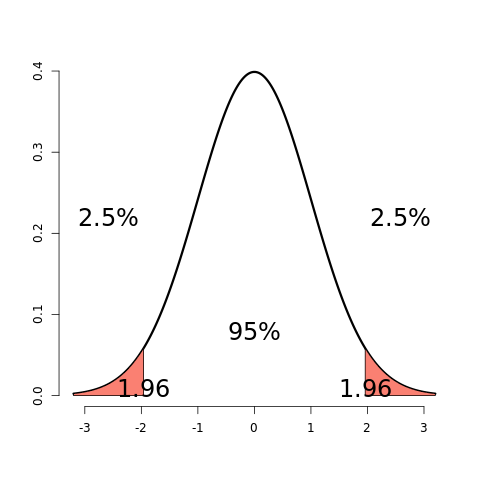
\includegraphics[scale = 0.4]{figs/two sided tail test.png}
    \caption{Two sided tail test presenting a standard normal $\mathcal{N}(0,1)$ distribution. We're going to reject $H_0$ if our test statistic is above $1.96$ -which has a 2.5\% chance under the null hypothesis- and we're going to reject $H_0$ if our test statistic is below $-1.96$ -which also has a 2.5\% chance under the null hypothesis-. Thus the union of those two events has a 5\% chance under the null hypothesis. }
    \label{fig:my_label}
\end{figure}

In hypothesis testing, we fix the $\alpha$ (type I error value) to be low. So if we reject the null hypothesis, either our model is wrong or there is a low probability that we made and error. We haven't fixed the probability of a type II error $\beta$, therefore we tend to say "fail to reject $H_0$" rather than accepting $H_0$. In general, less is known about the type II error. Statistical significance is not the same as scientific significance. 

\subsubsection{Two sided tests}

The Z-test requires the assumption of the Central Limit theorem and for $n$ to be large enough for the CLT to apply. If $n$ is mall, then a Gossett's $T$ test is performed exactly in the same way with the normal quantiles being replaced by the appropriate Student's $T$ quantiles and $n-1$ degrees of freedom. 

The probability of rejecting a false null hypothesis is called \textbf{power}. The statistical power of a dichotomic (binary) hypothesis test is the probability that the test correctly rejects the null hypothesis $H_0$ when a specific alternative hypothesis $H_1$ is true\footnote{Remember that the probability of rejecting a true null hypothesis is the type I error rate and is set to be small whilst the probability of failing to reject (this is the mistaken acceptance) a false null hypothesis is called a type II error rate. The power is $1-\beta$.}. A high value of power is good thing, we want to reject a false null hypothesis but it's not an easy to manipulate quantity in an experiment. One way to combat this issue is, prior to conducting the study, to do a power calculation of the sample size to obtain a certain level of power using guesses for the standard deviation and the hypothesised significant effect.

For example, suppose that $n=16$ (rather than 100) in our previous example. Instead of using a Z-test, we use a Student's $T$-test. Then 

$$
.05 = \mathds{P}\bigg(\frac{\Bar{X}-30}{s/\sqrt{16}} \geq t_{1-\alpha, 15} \bigg| \mu = 30\bigg)
$$

where $s/\sqrt{16}$ is the estimated standard error, where $t_{1-\alpha, 15}$ is t-quantile. Then our test statistic is now $\sqrt{16}\frac{32-30}{10} = .8$, while the critical value is $t_{1-\alpha, 15} = 1.75$. Thus, we fail to reject the null hypothesis. Remember that T has a heavier tail distribution than the normal distribution.

We are now interested in a two sided test. We are interested in studying if our hypothesised mean is significantly larger than $30$ or significantly smaller than $30$. That is, we want to test he alternative hypothesis $H_a: \mu \neq 30$. Then

$$
\alpha = \mathds{P}\bigg(\bigg|\frac{\Bar{X}-30}{s/\sqrt{16}}\bigg| > t_{1-\alpha/2, 15}\bigg| \mu = 30\bigg),
$$

that is: we'll reject $H_0$ is the test statistic (0.8) is either too large or two small with the critical value being calculated using $\alpha/2$. In our example, this critical value is $2.13$ so we fail to reject it\footnote{We note that, if the data are iid Gaussians, then $\frac{X-\mu}{s/\sqrt{n}} \sim t_{n-1}$} The previous calculation can be understood with the following R routine 

\begin{lstlisting}[language=R]
xval <-  seq(-4, 4, length=1000)
yval <- dt(xval, 15)
plot(xval, yval, type = "l", axes=TRUE, frame=FALSE, lwd = 3, xlab="", ylab= "")
x <- seq(qt(.975, 15), 4, length=100)
polygon(c(x, rev(x)), c(dt(x,15), rep(0,length(x))), col="salmon")
text(mean(x), mean(dt(xval, 16-1))+0.2, "2.5%", cex=2)
text(qt(.975,15), .01, "2.13",cex=2)
x <- seq(-3.2, qt(.025,16), length=100)
polygon(c(x, rev(x)), c(dt(x,15), rep(0,length(x))), col="salmon")
text(mean(x), mean(dt(xval, 16-1))+0.2, "2.5%", cex=2)
text(qt(.025,15), .01, "2.13",cex=2)
text(0, dt(0,15)/5, "95%", cex=2)
\end{lstlisting}

which outputs figure \ref{fig: two sided Student's T test}. \\

\begin{figure}
    \centering
    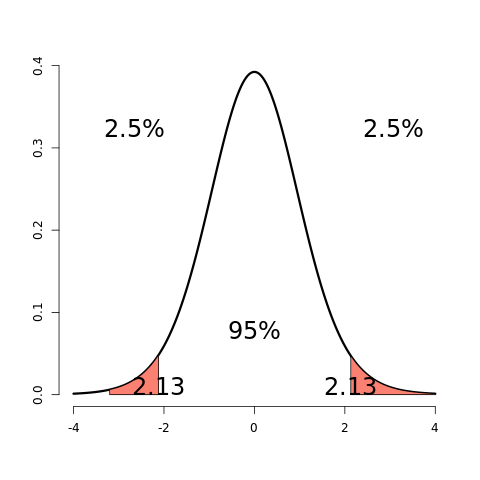
\includegraphics[scale=0.4]{figs/two sided T test.png}
    \caption{We calculate our normalised test statistic $\frac{\Bar{X}-\mu}{s/\sqrt{n}}$ and the probability that the absolute value of said statistic is bigger than $2.13$ \textit{ie.} the probability that the statistic is too large positive than $2.13$ is 2.5\% or too small negative than $-2.13$ is 2.5\%. In our case, the probability that the test statistic lies in the rejection region is 5\%. For the $T$ distributionwith 15 degrees of freedom, the 97.5th quantile is 2.13 and the 2.5th quantile is $-2.13$. }
    \label{fig: two sided Student's T test}
\end{figure}

\subsubsection{Confidence intervals and P values}

Consider testing $H_0 : \mu = \mu_0$ versus $H_a : \mu \neq \mu_0$. Take the set of all possible values for which we fail to reject $H_0$, this set is a $(1-\alpha)\times 10\%$ confidence interval for $\mu$, these are the value for $\mu$ that are supportable as null hypotheses (those are reasonable numbers for $\mu$). This rule works both ways, if a $(1-\alpha)\times 10\%$ contains $\mu_0$, then we fail to reject $H_0$.

Consider that we don't reject $H_0$ if our test statistic behaves as follows:

$$
\bigg|\frac{\Bar{X}-\mu}{s/\sqrt{n}}\bigg| \leq t_{1-\alpha/2, n-1},
$$

which implies 

$$
|\Bar{X}-\mu| \leq t_{1-\alpha/2, n-1} s/\sqrt{n}
$$

which, in turn, implies that 

$$
\bar{X} - t_{1-\alpha/2, n-1} \frac{s}{\sqrt{n}} < \mu_0 < \bar{X} + t_{1-\alpha/2, n-1} \frac{s}{\sqrt{n}}.
$$

This states that if $\mu_0$ lies inside the confidence interval, the we've failed to reject $H_0$ and this argument is reversible. This establishes a duality between confidence intervals and two-sided hypotheses tests. If we create a 95\% confidence interval, it conveys more information than the result of a hypothesis test because we can do the hypothesis test and gives a sense of what values for $\mu_0$ are well supported, helping to reduce the gap between statistical significance and scientific significance. 

In our previous example, we rejected the one-sided test when $\alpha = .05$, would we reject it if $.01$ or $.001$?

The smallest value for $\alpha$ that you still reject the null hypothesis is called the \textbf{attained significance level}. This equivalent, but philosophically different, from the \textbf{P-value}.
The P-value (same number but different concept) is the probability, under the null hypothesis, of obtaining evidence as extreme or more extreme than would be observed by chance alone, where chance is governed by the null distribution. If the P-value is small, then either $H_0$ is true and we have observed a rare event, given that the null hypothesis is true, or $H_0$ is false. It quantifies whether or not getting a test statistic as or more extreme than you observed was rare under the null hypothesis. If it's rare, then that casts some doubt on the veracity of the null hypothesis. 

In our example, the $T$ statistic was $0.8$. What's the probability of getting a $T$ statistic as large as $0.8$? This can be computed with the following R code 

\begin{lstlisting}[language=R]
pt(0.8, 15, lower.tail = FALSE) 

In [1]:  0.218099
\end{lstlisting}

where \texttt{pt} stands for $T$ probability, \texttt{lower.tail = FALSE} indicates we want a value above $0.8$, not lower. This works out to be $P = 22\% > \alpha = 5\%$, which is entirely reasonable because we failed to reject the null hypothesis. 

\begin{itemize}
    \item If the P-value is larger than $\alpha$, we fail to reject $H_0$. 
    \item If the P-value is smaller than $\alpha$, we reject $H_0$
\end{itemize}

This can be understood via the following R routine 

\begin{lstlisting}[language=R]
pt(0.8, 15, lower.tail=FALSE)
xval <-  seq(-4, 4, length=1000)
yval <- dt(xval, 15)
plot(xval, yval, type = "l", axes=TRUE, frame=FALSE, lwd = 3, xlab="", ylab= "")
x <-  seq(.8, 4, length=100)
polygon(c(x, rev(x)), c(dt(x,15), rep(0,length(x))), col="salmon")
text(mean(x), mean(dt(xval, 16-1))+0.2, "22%", cex=2)
text(.8, .01, "0.8",cex=2)
\end{lstlisting}

which outputs figure \ref{fig: P-value T statistic}.

\begin{figure}
    \centering
    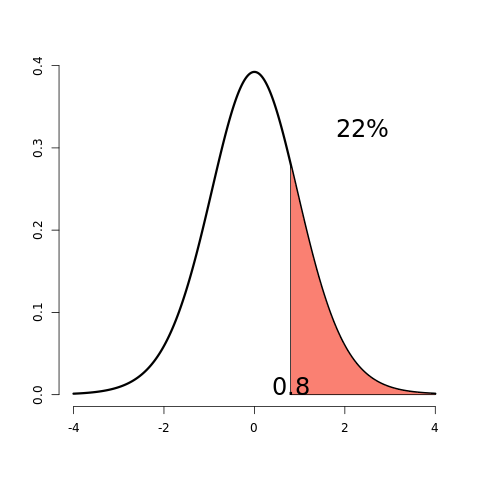
\includegraphics[scale = .4]{figs/P-value T statistic.png}
    \caption{Our statistic $\frac{\bar{X}-\mu}{s/\sqrt{n}}$ turned out to be .8. The probability of being .8 or larger for a Student's $T$ distribution with 15 degrees of freedom is $22\%$. Since this number is larger than $\alpha = 5\%$, we would fail to reject $H_0$. }
    \label{fig: P-value T statistic}
\end{figure}

By reporting a P-value, the reader can perform a hypothesis test at whatever $\alpha$ level he or she chooses. Again, is the P-value is less than $\alpha$, we reject the null hypothesis.

For two sided hypothesis test, double the smaller of the two one sided hypothesis test P-values. \\ 

Criticisms of the P value:

\begin{itemize}
    \item P values only consider significance, unlike confidence intervals making it harder to distinguish practical significance from statistical significance.
    \item Absolute measures of the rareness of an event are not good measures of the evidence for or against a hypothesis.
\end{itemize}

\subsubsection{Power}

Power is the probability of rejecting the null hypothesis when it's false. And, as the name suggests, it's a desirable quality, the more power, the more reliable the test is. A type II error is failing to reject the null hypothesis when it's false. Thus, by their definitions, power + type II error rate ($\beta$) sum to one. Thus we define $\textnormal{Power} = 1- \beta$.

Consider the example involving RDI. The null hypothesis is $H_0 : \mu = 30$ versus $H_a : \mu > 30$. Then power is calculated under the alternative hypothesis, as follows  

$$
\mathds{P}\bigg(\frac{\bar{X}-30}{s/\sqrt{n}} > t_{1-\alpha, n-1} \bigg | \mu = \mu_a\bigg).
$$

The power of the test is the probability that the $T$ statistic lies in the rejection region. If this normalised mean was greater than the $t_{1-\alpha, n-1}$ quantile, then we reject the null hypothesis. Note that this quantity is calculated not under the assumption of the null hypothesis but rather calculated under the assumption of the alternative hypothesis. Note that this function depends on the specific value of $\mu_a$ and we notice that, as $\mu \rightarrow 30$, power approaches $\alpha$. 

\clearpage

\subsubsection{Calculating Power}

Assume that $n$ is large, thus the central limit theorem holds - allowing us to use standard normal calculations rather than $T$ calculations-, and we know $\sigma$, then

\begin{align*}
    1- \beta = \mathds{P}\bigg(\frac{\bar{X}-30}{\sigma/\sqrt{n}} > z_{1-\alpha}\bigg|\mu = \mu_a\bigg) \\
    &= \mathds{P}\bigg(\frac{\bar{X}-\mu_a+\mu_a-30}{\sigma/\sqrt{n}}\bigg| \mu = \mu_a\bigg) \\
    &= \mathds{P}\bigg(\frac{\bar{X}-\mu_a}{\sigma/\sqrt{n}}> z_{1-\alpha}-\frac{\mu_a-30}{\sigma/\sqrt{n}}\bigg|\mu = \mu_a\bigg) \\
    &= \mathds{P}\bigg(Z > z_{1-\alpha} -\frac{\mu_a-30}{\sigma/\sqrt{n}} \bigg|\mu = \mu_a\bigg)
\end{align*}

In the first line we have our test statistic, $(\frac{\bar{X}-30}{\sigma/\sqrt{n}}$, which under the null hypothesis $H_0 : \mu = 30$ is a $Z$-statistic, but we are going to calculate it under the alternative hypothesis. Hence, our rejection region will be for the normalised mean values larger than a standard normal quantile. Then $1-\beta$ is the probability we reject a false null hypothesis, it's the probability that the statistic is larger than the quantile (the cutoff value), given that $\mu$ is in fact $\mu_a$. 
Since we are considering the alternative hypothesis and not the null hypothesis, this quantity -$(\frac{\bar{X}-30}{\sigma/\sqrt{n}}$- is no longer a $Z$-statistic but it's normal should the data be iid Gaussian. 

In line 2, we convert it into a $Z$-statistic by adding and subtracting $\mu_a$. In line 3 we take the correctly normalised mean $\frac{\bar{X}-\mu_a}{\sigma/\sqrt{n}} \sim \mathcal{N}(0, 1)$ which is in fact a $Z$-statistic (under the alternative hypothesis), and we calculate the probability that said quantity is larger than $z_{1-\alpha}-\frac{\mu_a-30}{\sigma/\sqrt{n}}$. 
In line 4, we calculate the probability of $Z$ being larger than $z_{1-\alpha}-\frac{\mu_a-30}{\sigma/\sqrt{n}}$, which can be easily computed provided $\sigma$ is known and a $\mu_a$ value has been selected. \\

\begin{tcolorbox}[title=Example]

\textbf{Statement}: Suppose we wanted to detect an increase in mean RDI of at least 2 events/hours above 30. Assume normality and setting a type I error rate of 5\% and that the sample in question will have a standard deviation of 4, what would be the power if we took a sample size of 16?

Now, $Z_{1-\alpha} = 1.645$ and $\frac{\mu_a-30}{\sigma/\sqrt{n}} = 2$. Then $\mathds{P}(Z > 1.645 - 2)  = \mathds{P}(Z > -0.355) = 64\%$

So under these settings, the probability of detecting an alternative of two events above the hypothesised value per hour is 64\%. Note that this is only a bound for all values above 32\%, the power gets larger as the alternative goes away from 30 events per hour.

\end{tcolorbox}

\begin{tcolorbox}[title=Example of a Sample Size Calculation]
Suppose we have a power we want to achieve for a particular value of the alternative, what sample size would we need to achieve it? What $n$ would be required to get a power of 80\%?

We want to compute the following expression and solve for $n$

$$
0.8 = \mathds{P}\bigg(Z > z_{1-\alpha} -\frac{\mu_a-30}{\sigma/\sqrt{n}} \bigg|\mu = \mu_a\bigg)
$$

where the $Z$-statistic is in fact normalised under the alternative hypothesis. We set $z_{1-\alpha} -\frac{\mu_a-30}{\sigma/\sqrt{n}}  = z_{0.20}$, the 20th quantile of the standard normal distribution and solve for $n$. This guarantees a 80\% or higher power, so $\mu_a$ is typically the smallest effect which can be reasonably detected. The calculation for $H_a: \mu < \mu_0$ is similar. 
\end{tcolorbox}

In general, for $H_a : \mu \neq \mu_0$ we calculate the one sided power using $\alpha/2$ (this is only approximately right since it excludes the probability of getting a large TS in the opposite direction of the truth).

In conclusion

\begin{itemize}
    \item Power goes up as $\alpha$ gets larger, \item Power of a one sided test is greater than the power of the associated two sided test,
    \item Power goes up as $\mu_1$ gets further away from $\mu_0$ and power goes up as $n$ goes up.
\end{itemize}

Regarding the first item, if we're requiring less evidence to reject the null hypothesis, we're bound to detect more alternative hypotheses. 

\clearpage

\subsubsection{T Tests and Monte Carlo}

\paragraph{\textbf{Power for the T test}}: Consider calculating power for a Gossett's $T$ test for our example. The power is 
\begin{align*}
\mathds{P}\bigg(\frac{\bar{X}-30}{S/\sqrt{n}}>t_{1-\alpha, n-1}\bigg|\mu = \mu_a\bigg)  = \mathds{P}\bigg(\sqrt{n}(\bar{X}-30)>t_{1-\alpha, n-1}S\bigg| \mu = \mu_a \bigg) \\
&= \mathds{P}\bigg(\frac{\sqrt{n}(\bar{X}-30)}{{\sigma}}>t_{1-\alpha, n-1}\frac{S}{\sigma}\bigg| \mu = \mu_a \bigg) \\
&= \mathds{P}\bigg(\frac{\sqrt{n}(\bar{X}-\mu_{a})}{{\sigma}}+\frac{\sqrt{n}(\mu_{a}-30)}{{\sigma}}>\frac{t_{1-\alpha, n-1}}{\sqrt{n-1}}\times \sqrt{\frac{(n-1)S^2}{\sigma^2}}\bigg| \mu = \mu_a \bigg) \\
&= \mathds{P}\bigg(Z+\frac{\sqrt{n}(\mu_{a}-30)}{{\sigma}}>\frac{t_{1-\alpha, n-1}}{\sqrt{n-1}} \sqrt{\chi^2_{n-1}}\bigg| \mu = \mu_a \bigg),
\end{align*}

where $Z \sim \mathcal{N}(0,1)$ is the independent standard normal and where $\chi^2_{n-1}$ is the chi-squared random variable with $n-1$ degrees of freedom. In regards to the first expression, the power is the probability that our test statistic lies in the rejection region and it's performed under the alternative hypothesis and, in regards to the second-to-last expression, if the data are iid Gaussian $\frac{(n-1)S^2}{\sigma^2} \sim \chi^2_{n-1}$ and can be computed with the Monte-Carlo method, by simulating pairs of $Z$ random variables and $\chi^2$ random variables and evaluating this inequality for every pair. Note that, in general, $\mu_a$ per sé needs not to be specified, what we need to know is how different is $\mu_a$ from $\mu_0$ in standard deviation units. This quantity, $\frac{\mu_a-\mu_0}{\sigma}$, is called an effect size is a unit free quantity. For example, a Monte Carlo simulation 
can be performed to calculate the last expression for the RDI example with the following R code

\begin{lstlisting}[language=R]
no_sim <- 100000 # number of simulation to perform 
n_dof <- 16 # number of degrees of freedom
sigma <- 4 # variance 
mu0 <- 30 # RDI mean under the null hypothesis
mua <- 32 # RDI mean under the alternative hypothesis
z <- rnorm(no_sim) # rnorm is the R function that simulates random variables having a specified normal distribution
chisq <- rchisq(no_sim, df = n_dof - 1) # chi squared distribution
t_qt <- qt(.95, n_dof-1) # 95th quantile for the Gossett's T distribution
mean(z + sqrt(n_dof)*(mua-mu0)/sigma > 
    t_qt/sqrt(n_dof-1)*sqrt(chisq))

In[1]: [1] 0.60517
In[2]: function (x, ...) 
In[3]: UseMethod("mean")
In[4]: <bytecode: 0x56366e096b50>
In[5]: <environment: namespace:base>
\end{lstlisting}

In the previous code snippet, we have a 100000 pairs of normal and chi squared random variables, generated with the \texttt{rnorm} and \texttt{rchisq} R-functions. The \texttt{mean(...)} function returns a vector of ones every time the LHS is bigger than the RHS and zeros every time the LHS is smaller than the RHS and computes the mean of said vector entries. The accuracy of this computation is upto $\mathcal{O}\bigg(\frac{1}{n^2}\bigg)$. 

\subsubsection{Two Sample Tests - Matched Data I}

When comparing two groups, first and foremost we want to determine whether observations are paired or not\footnote{For example, consider a medical trial of some medication. In one case we randomize that treatment to one group of test subjects and randomize a placebo to the other group of test subjects. This is not paired as the groups are distinct. An instance where the data are paired is, for example, administering the medication and the placebo in some random order for every test subject. Now the data is paired since some test subjects received both the treatment and the control.}. When dealing with a single set of paired data, one strategy is to take the difference between the paired observation and do a single one-sample $t$ test of $H_0 : \mu_d = 0$ versus $H_0 : \mu_d \neq 0$ (or one of the other two alternatives). The desired test statistic

$$
\frac{\bar{X}_d - \mu_{d0}}{S_d/\sqrt{n}}
$$

where $\mu_{d0}$ is the value under the null hypothesis (typically 0), where $n$ is the number of pairs of observations (and not the total number of observations themselves). This is called the \textbf{ordinary paired two-group t-test}. 

\subsubsection{Two Sample Tests - Matched Data II}

Let's consider an example of a paired $T$-test.

\begin{tcolorbox}[title=Example]
Consider Exam 1 and Exam 2 grades from a previous class. Is there any evidence that the second exam was easier or harder than the first? \\

Clearly, the data are paired since it's the same students measured twice. This question can be answered by examining if the mean of exam one is different from the mean of exam two. 
\end{tcolorbox}

In general, giver our data, we can compute this with the following R code 

\begin{lstlisting}[language=R]
diff <- test2 - test1  #pair difference
n <- sum(!is.na(diff)) #number of subjects: 49
mean(diff) #mean of the pair difference: 2.88
sd(diff) #standard deviation of the pair difference: 7.61
testStat <- sqrt(n) * (mean(diff) - 0)/sd(diff) #test Statistic: 2.65

#we get the p-value by multiplying the probability of getting a test statistic 
# as large or larger than 2.65 for a Gossett's T distribution with n-1 dof by two, since it's a two sided test
2 * pt(abs(testStat), n-1, lower.tail = FALSE) # Since we're working with 48 dof, there's little diference from calculating a pnorm or a pt

------

## or using the R function
t.test(diff)
\end{lstlisting}

In our case we get that there appears to be a difference between the means of exam 1 and exam 2. \footnote{Graphically this can be represented with a so called "Mean difference plot", first presented by Tukey and by J. Martin Bland \& Douglas G. Altman.}. \\

\subsubsection{Two Sample Tests - Regression to the Mean}

Francis Galton was the first to recognise that for matched data, high initial observations tended to be associated with lower second observations and low initial observations observations tended to be associated with higher second observations. For example, sons of very tall fathers tend to be a little shorter and fathers of very tall sons tend to be shorter. Another example would be that second exams for those who scored very high on a first exam tend to be a little lower. 

In order to explain this phenomena, consider plot \ref{fig: Matched data plot}. Imagine if the tests were completely random and the students were iid draws from said distribution, so the higher observations of the exam were random observations. So the probability of a second observation being that high is quite low, since it's more likely to be in the center of the distribution. Conversely, a very low test (something that had a very low probability of occurring given that it's already low), the probability of a second test being that low is small. And so if the pairs of observations are exactly noise, then you'll have a lot of regression in the mean. This is one extreme of complete variation and, for a given student, there's no trend between exam 1' score and exam 2' score.

Consider the other extreme, let's imagine that the test was a perfect adjudicator of student's abilities, that it is a perfectly calibrated instrument and that there is no noise. Then the student should ideally get exactly the same score on both exams. At which point, there'd be no variation around an identity line of Exam 2 v. Exam 1. This is an extreme of no variation where there is a 100\% correlation. Every other practical case lies somewhere in between those two extremes. 
\begin{figure}
    \centering
    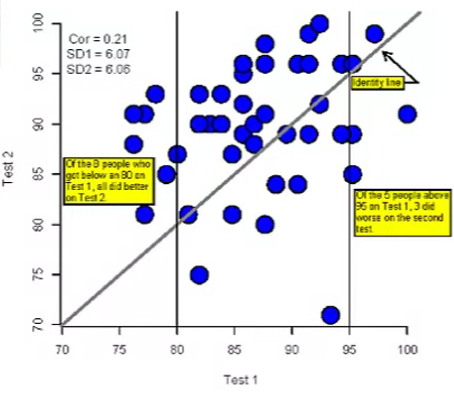
\includegraphics[scale = 0.4]{figs/Matched data plot.png}
    \caption{A matched data plot for the Exam 1 results v. Exam 2 results.}
    \label{fig: Matched data plot}
\end{figure}<

For example, of the eight people who got below 80 en the test, all did better on Test 2 and of the five people who got above a 95 test, three did worse on the second test. 

To investigate more, we normalise both scales (so that their empirical means are both 0 and their empirical standard deviations are 1). When asking questions about the paired data, we're asking questions about shifts in the means, information which we've gotten rid off. If there was no regression to the mean, the data would scatter about an identity line. The best fitting line goes through the average and has slope 

$$
\textnormal{Cor}(Test1, Test2) \frac{SD(Test2)}{SD(Test1)}
$$

and passes through the point 

$$
(\textnormal{mean}(Test1), \textnormal{mean}(Test2))
$$

Since we normalised the data, the best fitting line passes through (0,0) and has a slope of $\textnormal{Cor}(Test1, Test2) < 1$, since renormalizations don't affect the correlation. This will be shrunk toward a horizontal line, telling us our expected normalised test score for Test 2 is $\textnormal{Cor}(Test1, Test2)$ times the normalised Test 1 score. This line appropriately adjusts for regression to the mean for Test 2 conditioning on Test 1. We could similarly do the same for Test 1 conditioning on Test 2(in this case the best fitting line will have slope  
$\textnormal{Cor}(Test1, Test2)^{-1}$ if we plot with Test 1 on the Test 1 on the horizontal axis). The latter line will be shrunk toward a vertical line, the identity line will fall between the two. This can be better understood in plot \ref{fig: NTest2 v. NTest1}. In said plot we have the normalised Test 2 in the $y$-axis, the normalised Test 1 in the $x$-axis and the slope of the best regression line of Test 1 on Test 2 is the correlation between the two (0.21). In the middle we plot the identity line whilst the best regression line of Test 2 on Test 1 the slope is the inverse of the previous slope $1/0.2$. Note that all three lines pass through the (0,0).

\begin{figure}
    \centering
    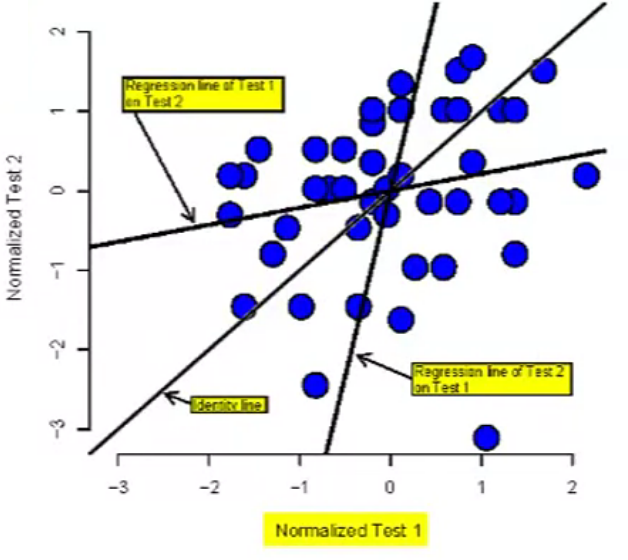
\includegraphics[scale=0.4]{figs/Normalised Test 2 v. Normalised Test 1 (adjusted).png}
    \caption{Normalised Test 2 scores v. Normalised Test 1 scores and the best fitting lines.  In this plot we have the normalised Test 2 in the $y$-axis, the normalised Test 1 in the $x$-axis and the slope of the best regression line of Test 1 on Test 2 is the correlation between the two (0.21). In the middle we plot the identity line whilst the best regression line of Test 2 on Test 1 the slope is the inverse of the previous slope $1/0.2$. Note that all three lines pass through the (0,0).}
    \label{fig: NTest2 v. NTest1}
\end{figure}

The line to be used when predicting test 2 scores from test 1 scores is a very flat (suggesting there's little correlation between the two tests, and this amount of noise also suggests there's a fair amount of regression to the mean) line whilst the line used to predict test 1 scores from test 2 scores is a very vertical line (because our correlation was quite low, suggesting a high amount of noise). Should the points collapse around an identity line, this suggests there's very little regression. 

In conclusion:

\begin{itemize}
    \item An ideal examiner would have little difference between the identity line and the fitted regression line.
    \item The more unrelated the two exam scores are the more pronounced the regression to the mean is.
\end{itemize} 

\subsubsection{Two Sample Tests - Two Independent Groups}

The extension to two independent groups is straightforward. Let $H_0 : \mu_1 = \mu_2$ versus $H_a: \mu_1 \neq \mu_2$ (or one of the other two alternatives). Assuming a common error variance we have that the following statistic

$$
\frac{\bar{X}-\bar{Y}}{S_p \sqrt{\frac{1}{n_X}+\frac{1}{n_Y}}} \sim t_{n_X+n_Y-2},
$$

under the null hypothesis $\bar{X}-\bar{Y}$ has a hypothesised mean of $0$ and if the data are iid Gaussian. In the limit of a large sample size, the previous statistic follows a normal distribution. If the assumption of a common error variance is questionable then 

$$
\frac{\bar{X}-\bar{Y}}{S_p \sqrt{\frac{1}{n_X}+\frac{1}{n_Y}}} \sim \mathcal{N}(0,1) \textnormal{ if } n_x, n_y \rightarrow \infty.
$$

where $S_p$ is the pooled variance. Furthermore, this statistic follows an approximate (only approximately, since the variances are not the same) Student's $T$ distribution if $X_i \sim \mathcal{N}(\mu_1,\sigma^2_1)$ and $Y_i \sim \mathcal{N}(\mu_2,\sigma^2_2)$. The approximate degrees of freedom are 

$$
\frac{(S_x^2/n_x+S_y^2/n_y)^2}{(S_x^2/n_x)^2/(n_x-1)+(S_y^2/n_y)^2/(n_y-1}
$$

where $S_x$ and $S_y$ are the variances within group 1 and group 2 respectively. 

Note that the connection between hypothesis testing and confidence intervals still holds: for example, if zero is in our independent group $T$ interval, we will fail to reject the independent group $T$ test for equal means and viceversa, if we construct a confidence interval by finding all of the hypothesised values for differences of means for which we fail to reject the null hypothesis we wind up with the appropriate $t$ confidence interval. 

If we want to test equality of means, in general it's incorrect constructing separate confidence intervals, one CI for group I and another CI for group II, and seeing if those CIs overlap. This procedure only works if the CIs don't overlap and we reject, this is an accurate statement. But the confidence intervals can overlap and the correctly constructed test statistic would still reject, seemingly leading to a contradiction.  This procedure has lower power than the correctly implemented test.

\begin{tcolorbox}[title=Exam]

Suppose that instead of having repeated data on two consecutive exams, students were randomised to two teaching modules and took the same exam. We treat the data as independent group data. We might obtain data like the following 

Group || N || Mean Exam || SD
Exam
Module 1 || 50 || 86.9 || 6.07
Module 2 || 50 || 89.8 || 6.06

The pooled standard deviation is 6.065 and the test statistic is 

$$
\frac{89.8-86.9}{6.065\sqrt{\frac{1}{50}+\frac{1}{50}}}
$$
\end{tcolorbox}

Suppose you have equal numbers of observations for two groups, $X$ and $Y$. If the data are truly matched, then the standard error of the difference is estimating 

$$
\sqrt{\frac{\sigma_x^2}{n}+\frac{\sigma_y^2}{n}-2\frac{\textnormal{Cov}(X,Y)}{n}}.
$$

If we ignore the matching by setting $\textnormal{Cov}(X,Y) = 0$, the standard error of the difference is estimating is estimating

$$
\sqrt{\frac{\sigma_x^2}{n}+\frac{\sigma_y^2}{n}}{n}.
$$

Since, generally, matched data is positively correlated, by ignoring the matching, we are unnecessarily augmenting the standard error. 

\end{document}
